%
\documentclass[%
 reprint,
 amsmath,amssymb,
 aps,
]{revtex4-1}

\usepackage{graphicx}% Include figure files
\usepackage{dcolumn}% Align table columns on decimal point
\usepackage{bm}% bold math


\begin{document}


\title{ APRENDIZAJE SUPERVISADO}
\author{Damian Mamani, David Reynaldo| Mamani Limache, Jhony| Mamani Maquera, Jorge Luis| Nombre}
		
\affiliation{%
 Universidad Privada de Tacna \textbackslash Facultad de Ingenieria \textbackslash Escuela Profesional de Ingenieria de Sistemas
}%

\begin{abstract}
\begin{center}
\textbf{Resumen}
\end{center}
El presente articulo tiene como finalidad dar a conocer los diferentes conceptos y algortimos del Aprendizaje Supervisado lo cual perimite comprender la suficiente metodología estadística para poder aprovechar los algoritmos de aprendizaje automático, lo cuales se encuentran en la biblioteca scikit-learn de Python y luego aplicar este conocimiento para resolver un problema clásico de aprendizaje automático.
\\

\begin{center}
\textbf{Abstract}
\end{center}
The purpose of this article is to present the different concepts and algorithms of Supervised Learning, which allows us to understand enough statistical methodology to take advantage of machine learning algorithms, which are found in the Python scikit-learn library and then apply this knowledge to solve a classic machine learning problem.
\\
\end{abstract}



\maketitle

%\tableofcontents

\section {Introducción}\label{sec:1}
La primera modalidad de aprendizaje que tiene el machine learning es la de aprendizaje supervisado. Usándola, se entrena al algoritmo otorgándole las preguntas, denominadas características, y las respuestas, denominadas etiquetas. Esto se hace con la finalidad de que el algoritmo las combine y pueda hacer predicciones.\\\\
Según se comentó en el primer artículo de esta serie, la clasificación es una subcategoría del aprendizaje supervisado en la que el objetivo es predecir las etiquetas de clase categóricas (discreta, valores no ordenados, pertenencia a grupo) de las nuevas instancias, basándonos en observaciones pasadas.\\
Esquema general de un modelo de aprendizaje supervisado
\begin{center}
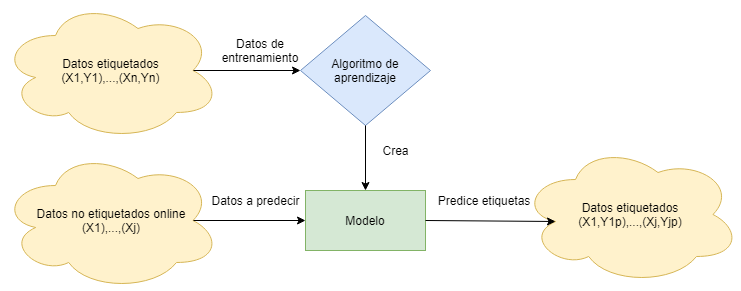
\includegraphics[width=7cm]{./Imagenes/esquemageneraldelmodelosupervisado}
\end{center}
 
Existen, a su vez, dos tipos de aprendizaje supervisado:\\
 \textbf{Regresión : }tiene como resultado un número específico. Si las etiquetas suelen ser un valor numérico, mediante las variables de las características, se pueden obtener dígitos como dato resultante.\\
 
 
\begin{center}
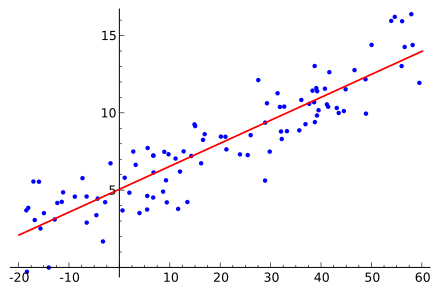
\includegraphics[width=7cm]{./Imagenes/regresion}
\end{center}
 
 \textbf{Clasificación : }en este tipo, el algoritmo encuentra diferentes patrones y tiene por objetivo clasificar los elementos en diferentes grupos.\\
 
 \begin{center}
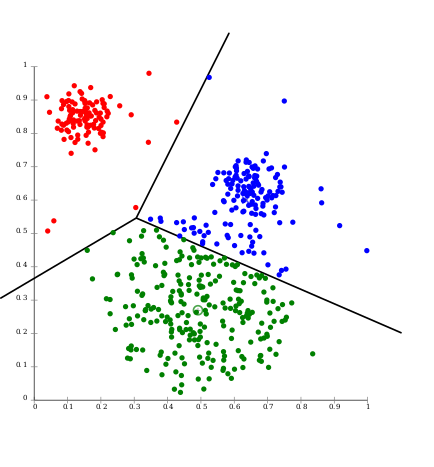
\includegraphics[width=7cm]{./Imagenes/clasificacion}
\end{center}

El algoritmo no está en capacidad de determinar a qué grupo pertenece un valor o cuál es el resultado de una operación. Solamente logra relacionar características con etiquetas y así obtener un resultado.\\

Hay dos tipos principales de clasificaciones:\\

 \textbf{Clasificación Binaria :} Es un tipo de clasificación en el que tan solo se pueden asignar dos clases diferentes (0 o 1). El ejemplo típico es la detección de email spam, en la que cada email es: spam  en cuyo caso será etiquetado con un 1 ; o no lo es  etiquetado con un 0.
  \textbf{Clasificación Multi-clase :}Se pueden asignar múltiples categorías a las observaciones. Como el reconocimiento de caracteres de escritura manual de números (en el que las clases van de 0 a 9).

 
%-----------------------------------------------------------------
\section{Objetivos}\label{sec:2}
\subsection{General:}
los algoritmos trabajan con datos “etiquetados” (labeled data), intentado encontrar una función que, dadas las variables de entrada (input data), les asigne la etiqueta de salida adecuada. El algoritmo se entrena con un “histórico” de datos y así “aprende” a asignar la etiqueta de salida adecuada a un nuevo valor, es decir, predice el valor da salida.

\subsection{Específicos:}
El aprendizaje supervisado se llama así porque el desarrollador actúa como una guía para enseñar al algoritmo las conclusiones a las que debe llegar, es decir la salida del algoritmo ya es conocida. Es similar a la forma en que un niño podría aprender de un maestro.
 \begin{center}
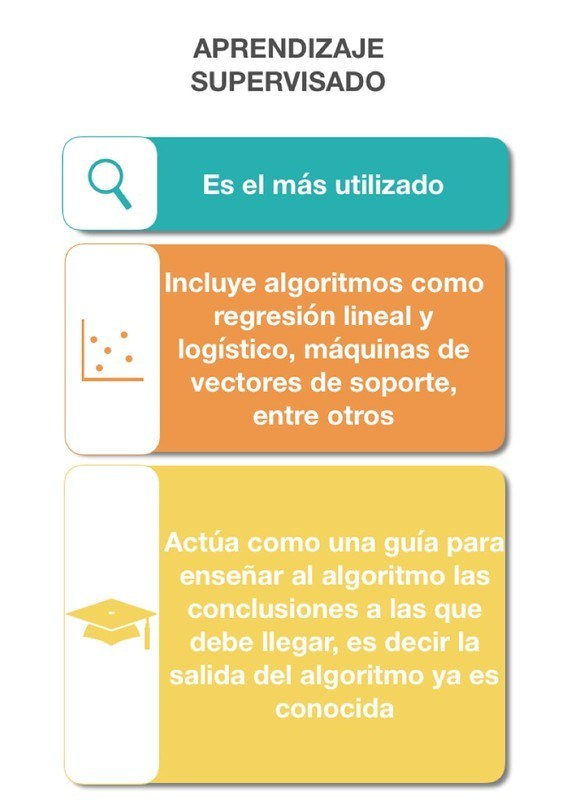
\includegraphics[width=5cm]{./Imagenes/objetivoprincipal}
\end{center}


%-----------------------------------------------------------------
\section {Marco Teórico}

\subsection{¿Que es aprendizaje supervisado?}	
 Son aquellos en los que producen funciones a partir de un conjunto de ejemplos de los que conocemos la salida deseada (dependiendo del tipo de salida, suele darse una subcategoría que diferencia entre modelos de clasificación, si la salida es un valor categórico, y modelos de regresión, si la salida es un valor de un espacio continuo).
La clave del aprendizaje automático son los algoritmos que pueden aplicarse a un
problema para poder dar una solución que no es evidente. El proceso se inicia cuando se reconoce
que con las técnicas de la estadística clásica no es suficiente para poder resolver el problema, y
entonces hay que abordarlo desde otro punto de vista, que consiste en confiar en que un algoritmo
pueda encontrar una solución mejor. (Hay quien dice que menos mala que la que nosotros tenemos).
el aprendizaje automático requiere un proceso de madurez continuo ya que todos
los algoritmos han funcionado al menos una vez muy bien con datos preparados, y muy
probablemente fallen con los datos que a nosotros nos interesa, aunque no por ello, haya que
desanimarse. La ciencia es un continuo proceso, que se recorre a veces a base de hipótesis que luego
resultan falsas: La gravedad era una fuerza según la mecánica clásica de Newton, y un espacio
deformado por los objetos según la teoría de la relatividad de Einstein. Dos conceptos totalmente
distintos.


%-------------------------------------------------
\subsection{Algoritmos que se usan en aprendizaje supervisado}	
 \textbf{Máquinas de Vector Soporte (SVM)}
Este algoritmo puede ser considerado una extensión del algoritmo “perceptron”. En SVM el objetivo de la optimización es establecer una línea de decisión que separe las clases maximizando el margen entre esta línea y los puntos de muestra cercanos a este hiperplano. Estos puntos se llaman vectores soporte.\\

\textbf{K-NN}
s un algoritmo de clasificación supervisado basado en criterios de vecindad. En particular, k-NN se basa en la idea de que los nuevos ejemplos serán clasificados según la clase a la cual pertenezca la mayor cantidad de vecinos más cercanos a ellos del conjunto de entrenamiento.

En particular, el algoritmo del vecino más cercano (aquel que asigna a una nueva muestra la clasificación de la muestra más cercana) explora todo el conocimiento almacenado en el conjunto de entrenamiento para determinar cuál será la clase a la que pertenece una nueva muestra, pero únicamente tiene en cuenta el vecino más próximo a ella, por lo que es lógico pensar que es posible que no se esté aprovechando de forma eficiente toda la información que se podría extraer del conjunto de entrenamiento.

Con el objetivo de resolver esta posible deficiencia surge la regla de los k vecinos más cercanos (k-NN), que es una extensión en la que se utiliza la información suministrada por los k ejemplos del conjunto de entrenamiento más cercanos al que queremos clasificar.\\
\textbf{Árbol de Decisión}
Los algoritmos de árbol de decisión desglosan el conjunto de datos mediante la formulación de preguntas hasta conseguir el fragmento de datos adecuado para hacer una predicción.

 \begin{center}
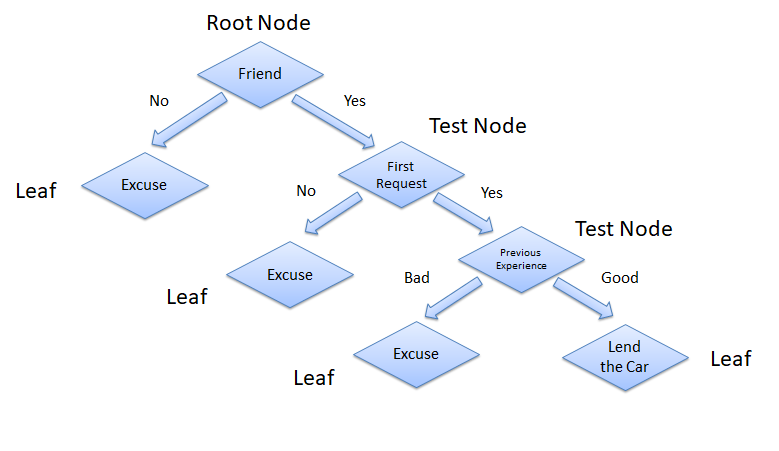
\includegraphics[width=7cm]{./Imagenes/arbol}
\end{center}
%-------------------------------------------------

\subsection{Aprendizaje supervisado por regresion y por clasificacion}

%-------------------------------------------------
\subsection{Ventajas,Desventajas e importancia}

  \textbf{VENTAJAS :}\\ • Es posible dar un algoritmo general para su aplicación. Es decir, se trata de un mecanismo muy bien definido, que no depende apenas del tipo de problema de clasificación al que nos enfrentamos. \\
  • Tenemos cierta seguridad sobre lo que puede hacer el clasificador y lo que no puede hacer.\\ • Durante el entrenamiento podemos medir el grado de acierto del clasificador y podemos detener el entrenamiento cuando lo consideremos aceptable.\\
  
    \textbf{DESVENTAJAS :} \\• Tenemos que el proceso de entrenamiento suele ser lento y no es infalible, se depende bastante de la elección de los casos de entrenamiento para que el clasificador sea capaz de generalizar lo suficiente.\\ • Es preciso un trabajo previo de clasificación manual de los casos que se usarán para el entrenamiento, que pueden ser muchos miles en un problema de cierta complejidad.\\
    
    \textbf{IMPORTANCIA :} \\
    El aprendizaje supervisado proporciona una ruta directa para convertir datos en información real y procesable. Al utilizar los datos como un recurso, les permite a las organizaciones comprender y prevenir los resultados no deseados o impulsar los resultados deseados para lo que sea que estén tratando de predecir.\\
    Por ejemplo, pueden decirle a una empresa que los clientes presentan un alto riesgo de agitación, la compañía puede llegar a ese cliente en particular con comunicaciones dirigidas y ofertas promocionales, lo que reduce su predisposición al abandono.\\
    Este aprendizaje es uno de los motores más potentes que permite que los sistemas de inteligencia artificial tomen decisiones empresariales de forma más rápida y precisa que los humanos.

 \begin{center}
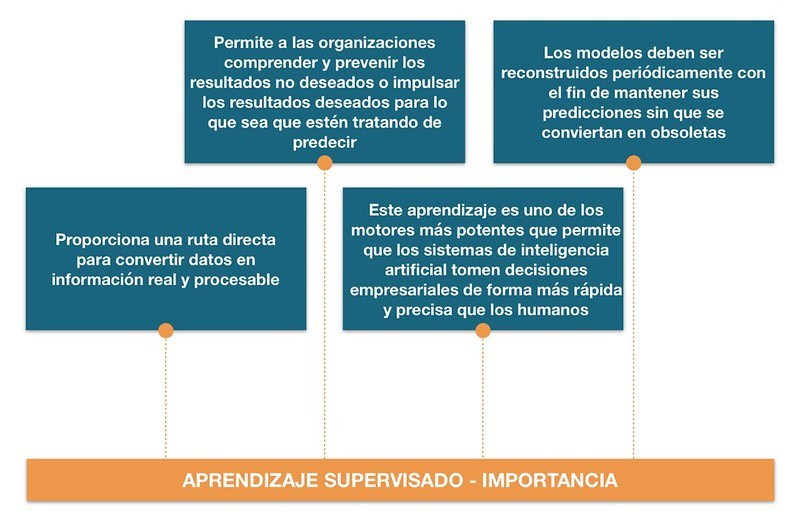
\includegraphics[width=7cm]{./Imagenes/importancia}
\end{center}

%-------------------------------------------------


\section{Ejemplo}

%-----------------------------------------------------------------
\section{Análisis}

La inteligencia, en pleno siglo XXI, trasciende las fronteras de la mente. Mucho escuchamos decir que ahora los computadores son más inteligentes que los cerebros y que pronto los robots sustituirán a los humanos para pasar a dominar el mundo.\\
Está muy arraigada la creencia de que por más inteligente que pueda ser un computador, nunca podrá tener la capacidad de pensar. Sin ánimos de fatalismo, el aprendizaje automático ha revolucionado de forma decisiva el campo de la computación, facilitando la realización de todo tipo de tareas de forma digital y no manual. \\
\\El aprendizaje automático, también conocido en inglés como machine learning, es un campo de la computación que lleva a otro nivel a la inteligencia artificial: hace que las computadoras aprendan a pensar.\\
\\
No, no es tan literal. Los computadores no desarrollaron un cerebro y ahora tienen emociones. Simplemente el machine learning desarrolla algoritmos que hacen que las máquinas puedan aprender por su cuenta y responder a determinadas preguntas con bastante certeza. Para desarrollar estos algoritmos, existen dos modalidades: aprendizaje supervisado y no supervisado.\\
\\
  \textbf{Aprendizaje supervisado: funcionamiento y tipos:} \\
La primera modalidad de aprendizaje que tiene el machine learning es la de aprendizaje supervisado. Usándola, se entrena al algoritmo otorgándole las preguntas, denominadas características, y las respuestas, denominadas etiquetas. Esto se hace con la finalidad de que el algoritmo las combine y pueda hacer predicciones.
Existen, a su vez, dos tipos de aprendizaje supervisado:
 \\
 \\
 \textbf{-  Regresión: }  tiene como resultado un número específico. Si las etiquetas suelen ser un valor numérico, mediante las variables de las características, se pueden obtener dígitos como dato resultante.
 \begin{center}
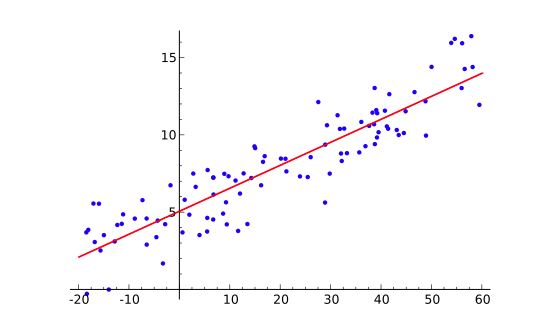
\includegraphics[width=8cm]{./Imagenes/regresion10}
\end{center}

 \textbf{}\\  
 \textbf{-  Clasificación: } 
: en este tipo, el algoritmo encuentra diferentes patrones y tiene por objetivo clasificar los elementos en diferentes grupos.
 \begin{center}
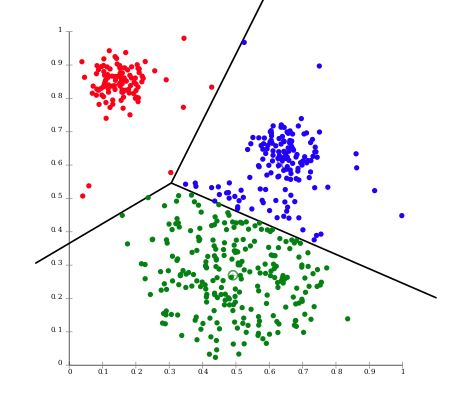
\includegraphics[width=8cm]{./Imagenes/clasificacion10}
\end{center}
El algoritmo no está en capacidad de determinar a qué grupo pertenece un valor o cuál es el resultado de una operación. Solamente logra relacionar características con etiquetas y así obtener un resultado.
 \textbf{}\\  
 \textbf{}\\  
\textbf{Aprendizaje no supervisado: ¿en qué consiste?} \\
A diferencia del aprendizaje supervisado, en el no supervisado solo se le otorgan las características, sin proporcionarle al algoritmo ninguna etiqueta. Su función es la agrupación, por lo que el algoritmo debería catalogar por similitud y poder crear grupos, sin tener la capacidad de definir cómo es cada individualidad de cada uno de los integrantes del grupo. \\
 \\
\textbf{¿Cómo se aplica esto en los softwares de automatización?} \\
El funcionamiento del machine learning y sus dos modalidades son muy fáciles de comprender. Pero, ¿cómo estos algoritmos pueden aplicarse en la vida real? Aunque cualquier particular puede desarrollar diferentes mecanismos simples y aplicarlos con algunos programas informáticos, lo mejor es obtener softwares que hagan todo el trabajo por ti, como los que ofrece WorkFusion.
\textbf{}\\  
\textbf{}\\  
\textbf{Diferencias entre el aprendizaje supervisado y el aprendizaje no supervisado} \\
\textbf{}\\  
\textbf{1. Datos de entrada en aprendizaje supervisado y aprendizaje no supervisado}\\  
\textbf{}\\  
La principal diferencia entre el aprendizaje supervisado y el aprendizaje no supervisado es la información utilizada en cualquiera de los métodos de aprendizaje automático. Vale la pena señalar que ambos métodos de aprendizaje automático requieren datos, que analizarán para producir ciertas funciones o grupos de datos. Sin embargo, los datos de entrada utilizados en el aprendizaje supervisado son bien conocidos y están etiquetados. Esto significa que la máquina solo tiene la función de determinar los patrones ocultos de los datos ya etiquetados. Sin embargo, los datos utilizados en el aprendizaje no supervisado no se conocen ni etiquetan. El trabajo de la máquina consiste en categorizar y etiquetar los datos brutos antes de determinar los patrones y funciones ocultos de los datos de entrada.
\textbf{}\\  
\textbf{}\\  
\textbf{2. Complejidad Computacional en Aprendizaje Supervisado y Aprendizaje No Supervisado}\\  
\textbf{}\\  
El aprendizaje automático es un asunto complejo y cualquier persona involucrada debe estar preparada para la tarea que le espera. Una de las diferencias sobresalientes entre el aprendizaje supervisado y el aprendizaje no supervisado es la complejidad computacional. Se dice que el aprendizaje supervisado es un método complejo de aprendizaje, mientras que el método de aprendizaje no supervisado es menos complejo. Una de las razones por las que el asunto del aprendizaje supervisado es el hecho de que uno tiene que entender y etiquetar las entradas mientras se está en el aprendizaje no supervisado, no se requiere que uno entienda y etiquete las entradas. Esto explica por qué muchas personas han estado prefiriendo el aprendizaje no supervisado en comparación con el método supervisado de aprendizaje automático.
\textbf{}\\  
\textbf{}\\  
\textbf{3. Precisión de los resultados del aprendizaje supervisado y el aprendizaje no supervisado}\\  
\textbf{}\\  
La otra diferencia que prevalece entre el aprendizaje supervisado y el aprendizaje no supervisado es la precisión de los resultados producidos después de cada ciclo de análisis de la máquina. Todos los resultados generados por el método supervisado de aprendizaje automático son más precisos y confiables en comparación con los resultados generados por el método de aprendizaje automático no supervisado. Uno de los factores que explica por qué el método supervisado de aprendizaje automático produce resultados precisos y confiables es porque los datos de entrada son bien conocidos y etiquetados, lo que significa que la máquina solo analizará los patrones ocultos. Esto es diferente al método de aprendizaje no supervisado donde la máquina tiene que definir y etiquetar los datos de entrada antes de determinar los patrones y funciones ocultos.
\textbf{}\\  
\textbf{}\\ 
\textbf{4. Número de clases en Aprendizaje Supervisado y Aprendizaje No Supervisado}\\   
\textbf{}\\ 
También vale la pena señalar que hay una diferencia significativa cuando se trata de la cantidad de clases. Vale la pena señalar que todas las clases utilizadas en el aprendizaje supervisado son conocidas, lo que significa que también es probable que se conozcan las respuestas en el análisis. El único objetivo del aprendizaje supervisado es, por lo tanto, determinar el grupo desconocido. Sin embargo, no hay conocimiento previo en el método de aprendizaje automático no supervisado. Además, se desconoce el número de clases, lo que significa claramente que no se conoce ninguna información y que los resultados se generan después de que no se puede determinar el análisis. Además, las personas involucradas en el método de aprendizaje no supervisado no conocen ninguna información relacionada con los datos en bruto y los resultados esperados.
\textbf{}\\  
\textbf{}\\ 
\textbf{5. Aprendizaje en tiempo real en aprendizaje supervisado y aprendizaje no supervisado}\\   
\textbf{}\\ 
Entre otras diferencias, existe el tiempo después del cual cada método de aprendizaje tiene lugar. Es importante resaltar que el método de aprendizaje supervisado se lleva a cabo fuera de línea mientras que el método de aprendizaje no supervisado se lleva a cabo en tiempo real. Las personas involucradas en la preparación y etiquetado de los datos de entrada lo hacen fuera de línea mientras que el análisis del patrón oculto se realiza en línea, lo que niega a las personas involucradas en el aprendizaje automático la oportunidad de interactuar con la máquina mientras analiza los datos discretos. Sin embargo, el método de aprendizaje automático no supervisado se lleva a cabo en tiempo real de manera que todos los datos de entrada se analizan y etiquetan en presencia de los alumnos, lo que les ayuda a comprender los diferentes métodos de aprendizaje y clasificación de los datos en bruto. El análisis de datos en tiempo real sigue siendo el mérito más importante del método de aprendizaje no supervisado.

\textbf{}\\  
\textbf{}\\ 
\textbf{TABLA QUE MUESTRA LAS DIFERENCIAS ENTRE EL APRENDIZAJE SUPERVISADO Y EL APRENDIZAJE NO SUPERVISADO: CUADRO DE COMPARACIÓN}\\  
\textbf{}\\ 
 \begin{center}
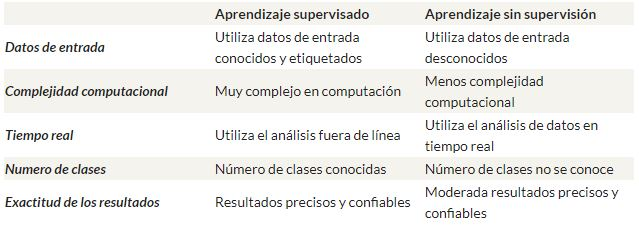
\includegraphics[width=9cm]{./Imagenes/tabla}
\end{center}
%-----------------------------------------------------------------
\section{Conclusiones}

\begin{itemize}
\item 
completar

\end{itemize}

\newpage
% Bibliografia.
%-----------------------------------------------------------------

\begin{thebibliography}{99}
http://machinelearningparatodos.com/tipos-de-aprendizaje-automatico/\\
https://www.toptal.com/machine-learning/explorando-algoritmos-de-aprendizaje-automatico-supervisado\\
https://medium.com/datos-y-ciencia/aprendizaje-supervisado-introducci%C3%B3n-a-la-clasificaci%C3%B3n-y-principales-algoritmos-dadee99c9407\\
https://medium.com/@juanzambrano/aprendizaje-supervisado-o-no-supervisado-39ccf1fd6e7b\\
http://ligdigonzalez.com/todo-sobre-aprendizaje-supervisado-en-machine-learning/\\
http://ligdigonzalez.com/diferencia-entre-aprendizaje-supervisado-y-no-supervisado/\\
https://empresas.blogthinkbig.com/que-algoritmo-elegir-en-ml-aprendizaje/\\



\end{thebibliography}


\end{document}
